\chapter{Tests und Experimente}
In diesem Kapitel werden Experimente mit den drei Datensätze durchgeführt. Ebenfalls werden verschiedene Hyperparameter getestet.

\section{Spiel-Datensatz Experimente}
Als erstes wird die Methode auf dem Spiel-Datensatz angewendet. Hiermit soll geprüft werden ob die Methode die erwartete
Ergebnisse liefert. Das U-Net wird für 100 Epochen mit Adam, eine Lernrate von 0.001 und die Cross Entropy Loss Funktion trainiert. Dieser
Einstellung erwies die besten Ergebnisse. Außerdem wurde ein Experiment mit 36 und ein mit 324 Bins durchgeführt, was kein Einfluss auf die 
Ergebnisse vorwies. Es kann davon ausgegangen werden, dass bei der niedrige Anzahl an möglichen Farben, ein Unterschied bei 36 und 324 Bins
nicht zu erkennen ist. Die unteren Ergebnissen wurden mit 324 Bins erstellt.

\begin{figure}[H]
  \vspace{1cm}
  \begin{subfigure}
    \centering
    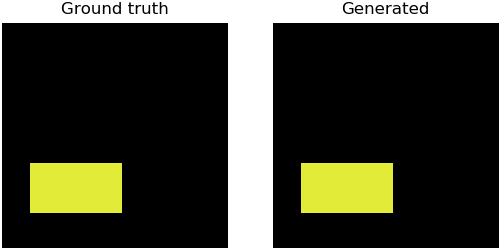
\includegraphics[width=.32\textwidth]{resources/experiments/30.png}
  \end{subfigure}
  \begin{subfigure}
    \centering
    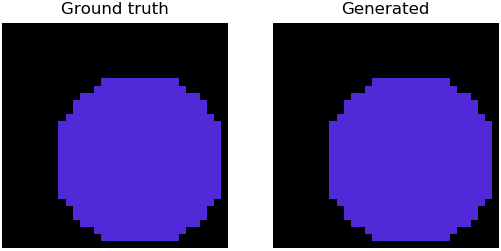
\includegraphics[width=.32\textwidth]{resources/experiments/31.png}
  \end{subfigure}
  \begin{subfigure}
    \centering
    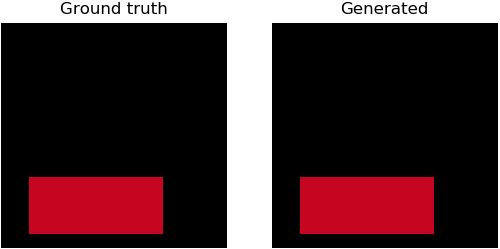
\includegraphics[width=.32\textwidth]{resources/experiments/42.png}
  \end{subfigure}
  \caption{Beispiele von sehr gute Ergebnisse aus dem Spiel-Datensatz}
  \label{image:gute-ergebnisse-toy-dataset}
\end{figure}

Bei den oberen Ergebnisse wurden alle Pixeln richtig klassifiziert, was bei der Größe des Datensatzes oft zu overfitting deutet.
Die unteren Ergebnissen zeigen dass das Model generalisiert und nicht overfitet hat.

\begin{figure}[H]
  \vspace{1cm}
  \begin{subfigure}
    \centering
    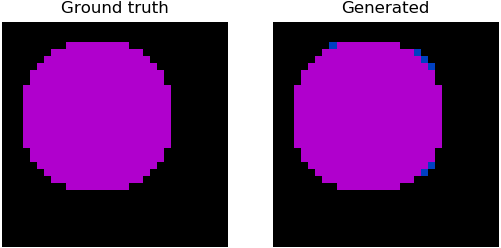
\includegraphics[width=.32\textwidth]{resources/experiments/581.png}
  \end{subfigure}
  \begin{subfigure}
    \centering
    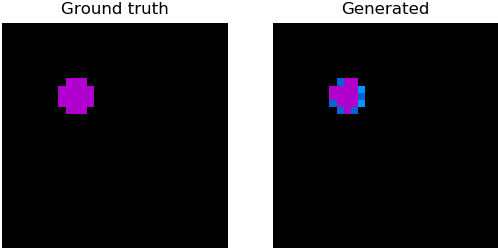
\includegraphics[width=.32\textwidth]{resources/experiments/712.png}
  \end{subfigure}
  \begin{subfigure}
    \centering
    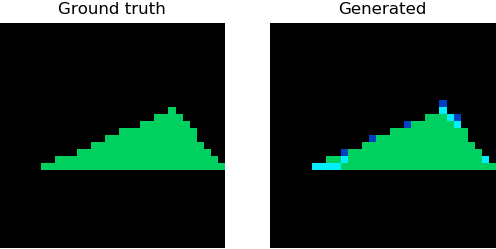
\includegraphics[width=.32\textwidth]{resources/experiments/761.png}
  \end{subfigure}
  \caption{Beispiele von generalisierte Ergebnisse}
  \label{image:nicht-gute-ergebnisse-toy-dataset}
\end{figure}

Das Model hat bei einige Ergebnisse, Schwierigkeiten die Pixeln am Rand der geometrische Formen, richtig zu klassifizieren.
Dies tritt speziell auf die Kreise und Dreiecke wo die Ränder nicht aus glatte Linien bestehen. Des weiteren wurden die Farben mittels
den Durchschnitt für jeden möglichen Bin über alle Farben von jeden Trainingsbild rekonstruiert.
\\
Die Ergebnisse bestätigen dass das Binning und die Methode funktionieren. Anschließend wurden Experimente auf komplexere Bilder
von dem Subset von CIFAR-100 durchgeführt.

\section{CIFAR-100 Subset Experimente}
Das Model wurde auf 12 Klassen von CIFAR-100 über 100 Epochen mit Adam, eine Lernrate von 0.001 und die Cross Entropy Loss Funktion
trainiert. Diese Einstellungen ergab sich als die beste Kombination von Hyperparameter, jedoch wurde das Training bei unter 50 Epochen unterbrochen
da der Validation Loss wieder gestiegen ist. Um diesen Anstieg zu vermeiden, wurde ein Mechanismus eingeführt um die Lernrate bei einem bestimmten
Faktor zu reduzieren wenn der Validation Loss nicht mehr sinkt oder sogar steigt. Dieser Mechanismus bietet PyTorch und wurde mit der 
Klasse \textit{ReduceLROnPlateau} implementiert.

\begin{figure}[H]
  \centering
  \vspace{1cm}
  \begin{subfigure}
    \centering
    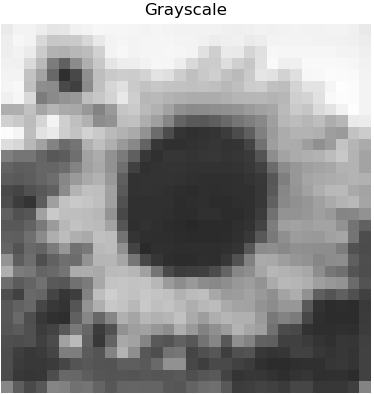
\includegraphics[width=.24\textwidth]{resources/experiments/cifar/200_grayscale.png}
  \end{subfigure}
  \begin{subfigure}
    \centering
    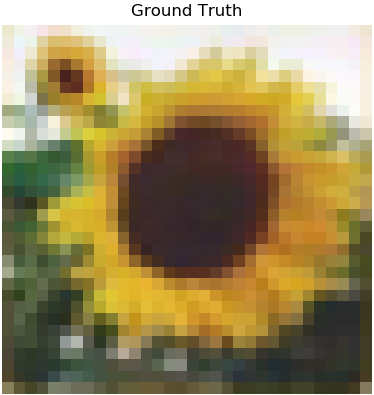
\includegraphics[width=.24\textwidth]{resources/experiments/cifar/200_original.png}
  \end{subfigure}
  \begin{subfigure}
    \centering
    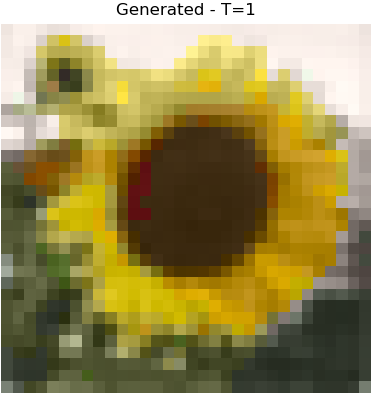
\includegraphics[width=.24\textwidth]{resources/experiments/cifar/200_t1.png}
  \end{subfigure}

  \begin{subfigure}
    \centering
    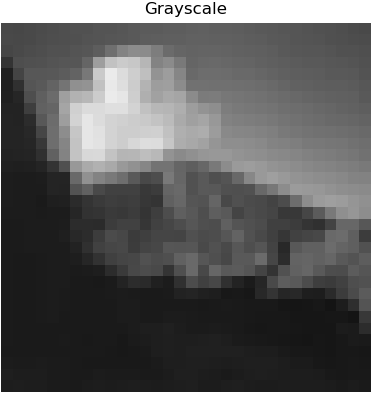
\includegraphics[width=.24\textwidth]{resources/experiments/cifar/600_grayscale.png}
  \end{subfigure}
  \begin{subfigure}
    \centering
    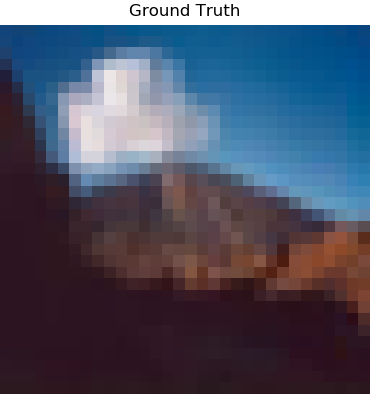
\includegraphics[width=.24\textwidth]{resources/experiments/cifar/600_original.png}
  \end{subfigure}
  \begin{subfigure}
    \centering
    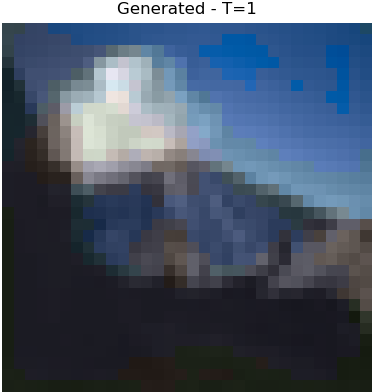
\includegraphics[width=.24\textwidth]{resources/experiments/cifar/600_t1.png}
  \end{subfigure}
  \caption{Beispiele von gute Ergebnisse aus dem Subset von CIFAR-100 mit 324 Bins. Die erste Spalte beinhaltet das Graustufenbild, die zweite Spalte
  beinhaltet das Originale Bild und die letzte Spalte stellt das generierte Bild dar. Das generierte Bild wurde mit eine Temperatur von 1
  erzeugt, was bedeutet dass die rekonstruierte Farben den Durchschnitt aus jedem Bin repräsentieren.}
  \label{image:gute-ergebnisse-cifar}
\end{figure}

Die Experimente mit diesem Datensatz haben gezeigt dass die Anzahl der Bins bei der Auswahl an möglichen Farben die Ergebnisse beeinträchtigen.
Eine Erhöhung an Trainingszeit zwischen 36 und 324 Bins war nicht zu erkennen.

% TODO: Change image
\begin{figure}[H]
  \centering
  \vspace{1cm}
  \begin{subfigure}
    \centering
    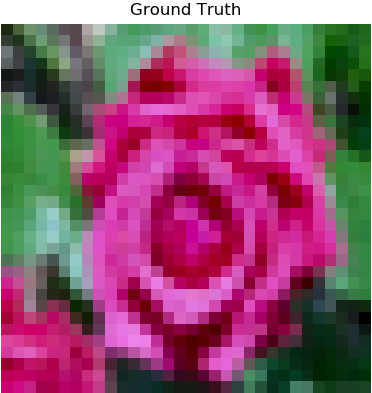
\includegraphics[width=.24\textwidth]{resources/experiments/cifar/12_original.png}
  \end{subfigure}
  \begin{subfigure}
    \centering
    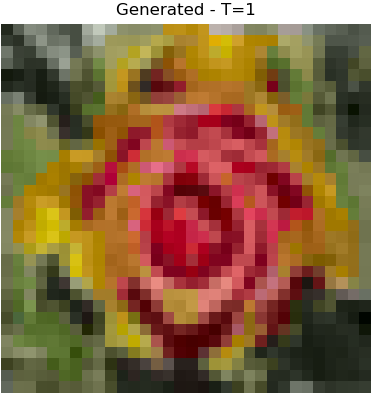
\includegraphics[width=.24\textwidth]{resources/experiments/cifar/12_t1.png}
  \end{subfigure}
  \begin{subfigure}
    \centering
    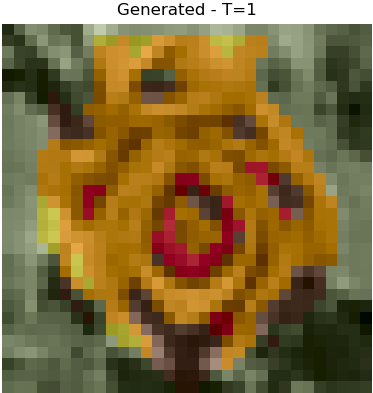
\includegraphics[width=.24\textwidth]{resources/experiments/cifar/12_t1_36.png}
  \end{subfigure}

  \caption{Einfluss von Anzahl der Bins auf die Ergebnisse. Das zweite Bild wurde mit 324 Bins generiert, das dritte nur mit 36.}
  \label{image:gute-ergebnisse-cifar}
\end{figure}

\subsection{Experimente mit MSE Loss und ohne Binning}
Um die Performance von Klassifikation gegenüber Regression zu messen, wurde ein Model mit der MSE Loss Funktion trainiert. Dieses Model
wurde ebenfalls mit den gleichen Parameter wie das Klassifikationsmodell trainiert und hat beeindruckende Ergebnisse erreicht. Einige Ergebnisse
zeigten Blasse stellen im Vergleich zu das Klassifikationsmodell, der leuchtende Farben an den gleichen Stellen gezeigt hat.

\begin{figure}[H]
  \centering
  \vspace{1cm}
  \begin{subfigure}
    \centering
    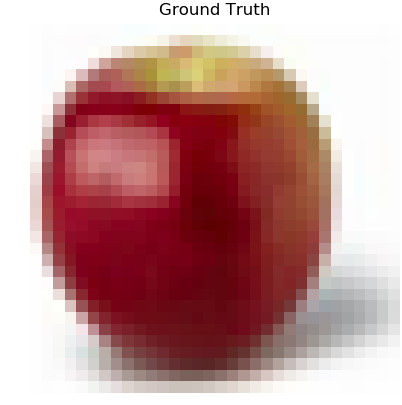
\includegraphics[width=.28\textwidth]{resources/experiments/cifar/311_original.png}
  \end{subfigure}
  \begin{subfigure}
    \centering
    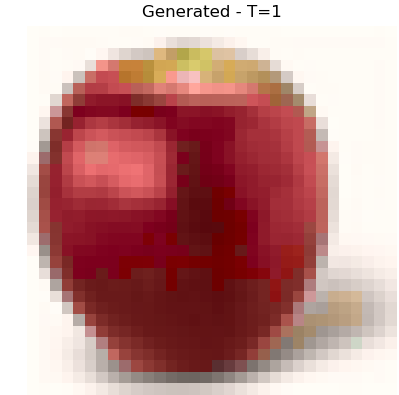
\includegraphics[width=.28\textwidth]{resources/experiments/cifar/311_t1.png}
  \end{subfigure}
  \begin{subfigure}
    \centering
    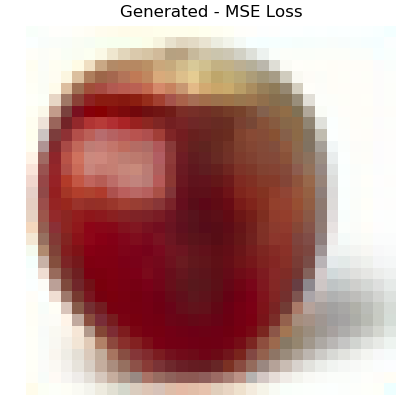
\includegraphics[width=.28\textwidth]{resources/experiments/cifar/311_regression.png}
  \end{subfigure}

  \caption{Vergleich von Klassifikation mit Binning gegenüber Regression. Das zweite Bild wurde mit 324 Bins generiert.
  Das dritte Bild wurde ohne Binning und mit einem MSE Loss generiert.}
  \label{image:gute-ergebnisse-cifar}
\end{figure}

\section{Landscape Datensatz Experimente}

% \begin{figure}[H]
%   \centering
%   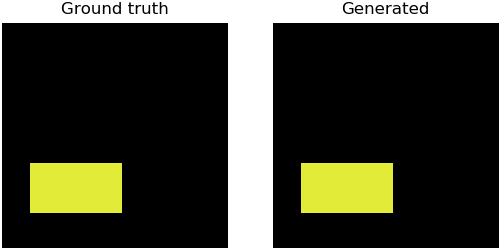
\includegraphics[width=1\textwidth]{resources/experiments/30.png}
%   \caption{
%   \gls{grid} mit 36 bins. Die x-Achse bildet die Werte von dem Farbkanal ``a'' und die y-Achse die Werte von den Farbkanal ``b'' ab.
%   }
%   \label{image:bins}
% \end{figure}